% Provenance (never printed): cycle 3 / 6e "La planete Terre, l'environnement
% et l'action humaine" (the Earth in the Solar System; conditions for life);
% see sources/book1/PROVENANCE.md. Book 1, grade 6, chapter 1.
\chapter{Bumi, Sebuah Planet dalam Tata Surya}\label{ch:g6:earth-a-planet}

Tiga wahana robot telah dikirim ke antariksa. Satu per satu, wahana-wahana
itu mengirimkan sebuah gambar ke Bumi, seperti kartu pos. Gambar pertama
datang dari Venus: sebuah bola pucat yang terbungkus \omterm{def:g4:clouds-rain-snow:cloud}{awan} tebal, tempat
udaranya cukup panas untuk melelehkan timah hitam dan menekan tanah dengan
berat yang meremukkan. Gambar kedua datang dari Mars: \omterm{def:g5:weather-and-climate:desert}{gurun} merah yang
dingin dan berdebu di bawah langit yang tipis. Wahana ketiga telah
mengarahkan kameranya kembali ke rumah: sebuah bola biru dan putih, dengan
\omterm{def:g2:water-on-earth:ocean}{samudra}, \omterm{def:g4:clouds-rain-snow:cloud}{awan}, dan es. Tiga planet, bertetangga di sekeliling Matahari yang
sama. Mengapa hanya satu di antaranya yang berwarna biru?
% ledger: nasa:venus-clouds, nasa:mars-water

\begin{omfigure}
\begin{minipage}[t]{0.31\linewidth}\centering
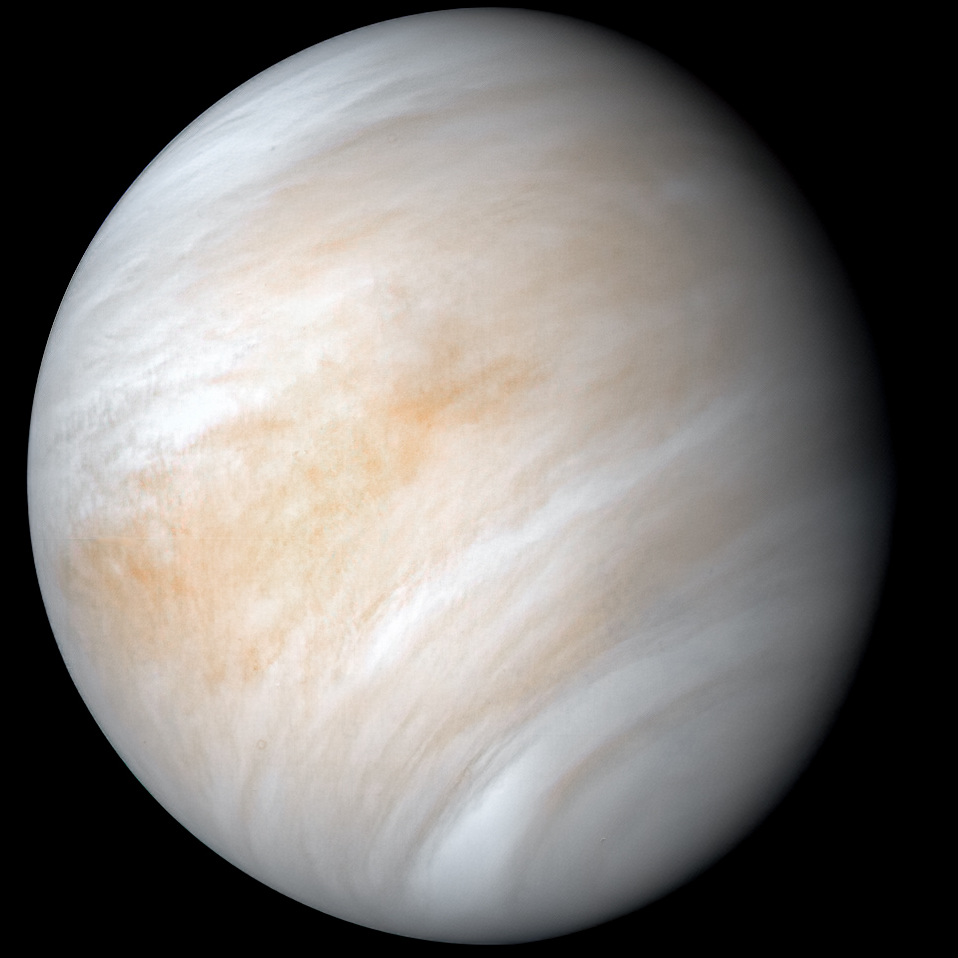
\includegraphics[width=\linewidth]{images/book1/g6-venus-mariner10.jpg}\\[2pt]
{\small Venus}
\end{minipage}\hfill
\begin{minipage}[t]{0.31\linewidth}\centering
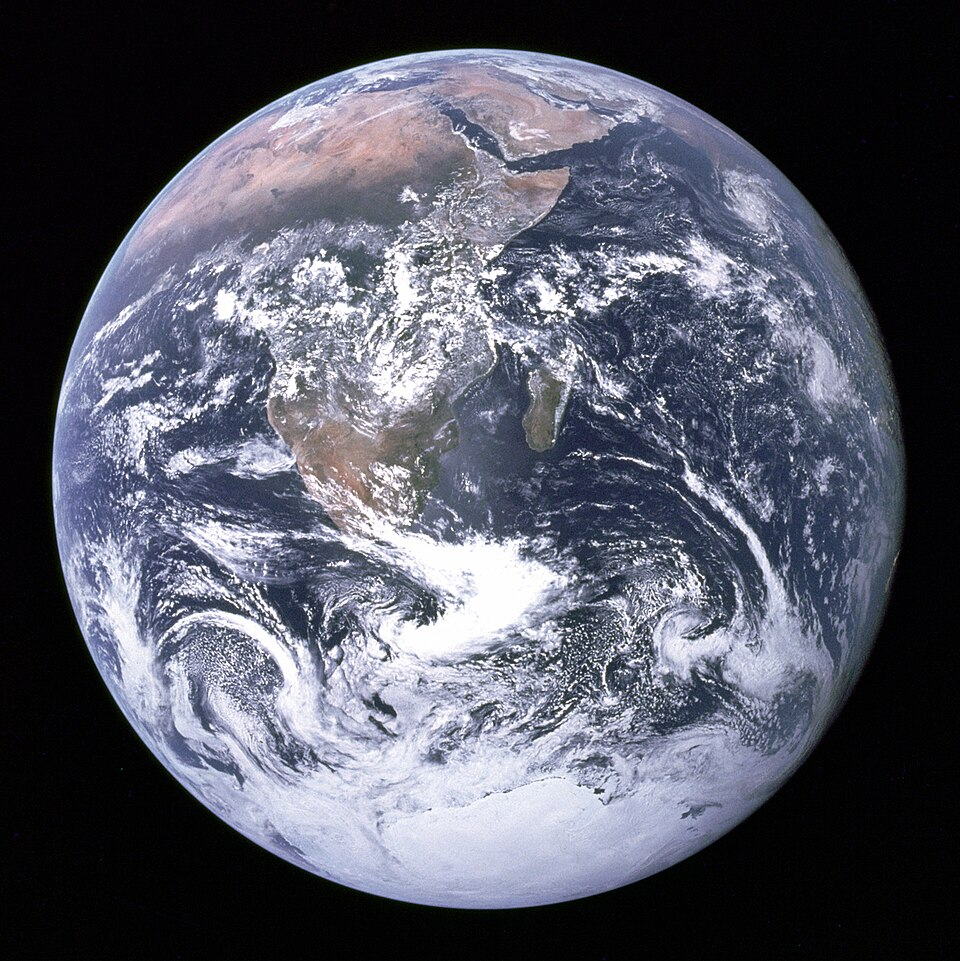
\includegraphics[width=\linewidth]{images/book1/g6-earth-apollo17.jpg}\\[2pt]
{\small Bumi}
\end{minipage}\hfill
\begin{minipage}[t]{0.31\linewidth}\centering
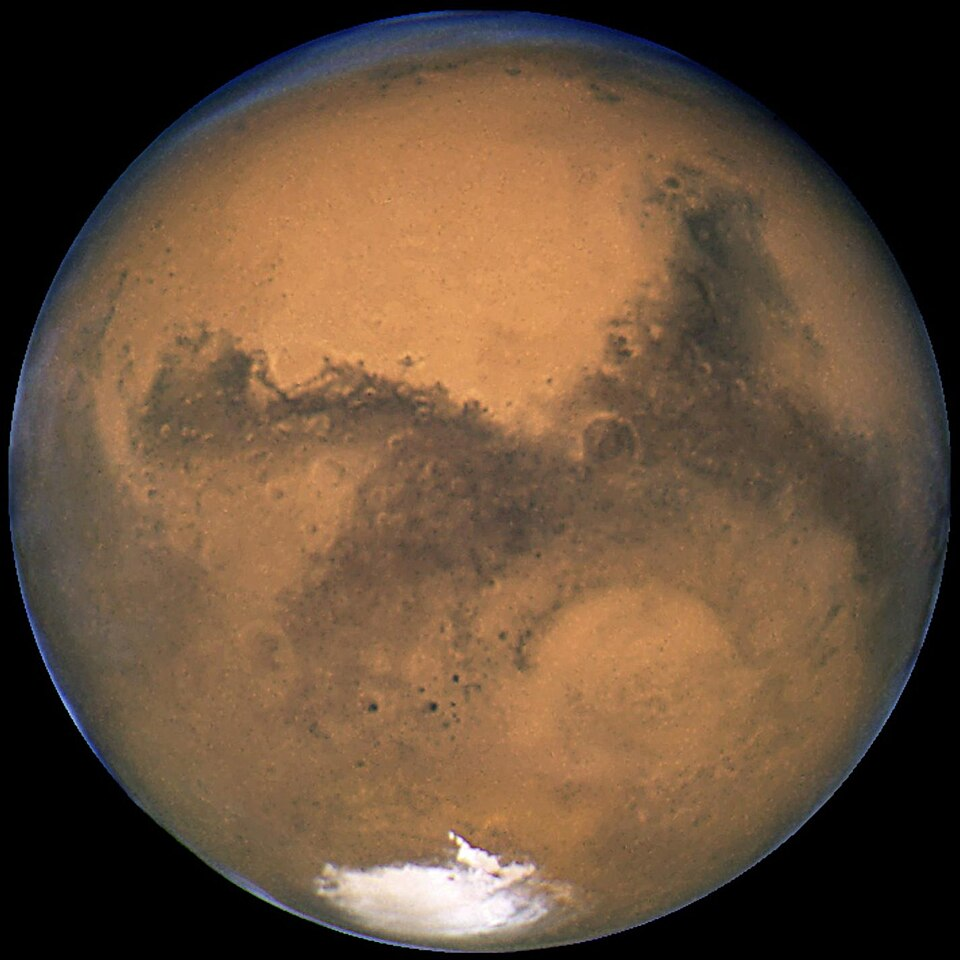
\includegraphics[width=\linewidth]{images/book1/g6-mars-hubble.jpg}\\[2pt]
{\small Mars}
\end{minipage}

\medskip
{\small Tiga kartu pos dari antariksa. Venus, difoto oleh wahana Mariner~10
pada tahun 1974: kita hanya melihat bagian atas \omterm{def:g4:clouds-rain-snow:cloud}{awannya}. Bumi, difoto oleh
awak Apollo~17 dalam perjalanan menuju Bulan pada tahun 1972: Afrika, Jazirah
Arab, dan es Antarktika di bawah \omterm{def:g4:clouds-rain-snow:cloud}{awan} putih. Mars, difoto oleh Teleskop
Antariksa Hubble pada tahun 2003, dengan tudung es putih di \omterm{def:g3:continents-and-oceans:poles}{kutubnya}.
(Foto: NASA/JPL-Caltech; NASA; NASA, ESA, dan Hubble Heritage Team.)}
% ledger: nasa:venus-mariner10, nasa:apollo17-earth, hubble:mars-2003
\end{omfigure}

\begin{recall}
Buku fisika telah menunjukkan bahwa Matahari adalah sebuah bintang, bola gas
panas raksasa yang bersinar sendiri, dan bahwa planet adalah benda besar
berbentuk bulat yang beredar mengelilingi sebuah bintang dan tidak bersinar
sendiri: kita melihatnya karena planet itu memantulkan cahaya bintangnya.
Matahari dan segala sesuatu yang beredar mengelilinginya membentuk Tata
Surya. Setiap planet beredar mengelilingi Matahari pada lintasan yang
disebut orbitnya, dan berputar pada dirinya sendiri di sekitar sebuah
sumbu. Udara di sekitar kita menekan segala sesuatu yang disentuhnya:
inilah tekanan udara. Massa jenis suatu bahan menunjukkan seberapa berat
volume tertentu dari bahan itu: satu sentimeter kubik air beratnya
1~gram, jadi massa jenisnya 1~gram per sentimeter kubik; bahan yang massa
jenisnya lebih besar daripada air tenggelam di dalam air, dan bahan yang
massa jenisnya lebih kecil terapung. Terakhir, kira-kira tujuh persepuluh
permukaan Bumi tertutup \omterm{def:g2:water-on-earth:ocean}{samudra}
(\cref{ch:g2:water-on-earth}).
\end{recall}

\section{Delapan planet mengelilingi Matahari}

Delapan planet beredar mengelilingi Matahari. Secara berurutan, dari yang
paling dekat sampai yang paling jauh, planet-planet itu adalah Merkurius,
Venus, Bumi, Mars, Jupiter, Saturnus, Uranus, dan Neptunus. Sebuah kalimat
dapat membantu mengingat urutannya: \emph{Makan Vitamin Bikin Mata Jadi
Sehat Untuk Nanti} (Merkurius, Venus, Bumi, Mars, Jupiter, Saturnus,
Uranus, Neptunus).

Gambar di bawah ini menunjukkan kedelapan planet berdampingan, digambar
dengan skala yang sama: jika sebuah planet dua kali lebih lebar daripada
planet lain, lingkarannya juga dua kali lebih lebar.

\begin{omfigure}
\pgfplotstableread{figdata/out/grade-6-planets-sizes.dat}\gsixsizes
\begin{tikzpicture}
  \draw[black!40] (-0.2,0) -- (13.8,0);
  \pgfplotstablegetrowsof{\gsixsizes}
  \pgfmathtruncatemacro{\gsixlast}{\pgfplotsretval-1}
  \foreach \i in {0,...,\gsixlast}{
    \pgfplotstablegetelem{\i}{x_cm}\of\gsixsizes \let\gx\pgfplotsretval
    \pgfplotstablegetelem{\i}{d_cm}\of\gsixsizes \let\gd\pgfplotsretval
    \def\gn{\ifcase\i Merkurius\or Venus\or Bumi\or Mars\or Jupiter\or Saturnus\or Uranus\or Neptunus\fi}
    \pgfplotstablegetelem{\i}{d_km}\of\gsixsizes \let\gk\pgfplotsretval
    \pgfmathsetmacro{\gr}{\gd/2}
    \ifnum\i<4
      \fill[brown!70!black, draw=black!60, line width=0.3pt] (\gx,\gr) circle (\gr);
    \else
      \fill[orange!35, draw=black!60, line width=0.3pt] (\gx,\gr) circle (\gr);
    \fi
    \node[font=\scriptsize, rotate=40, anchor=north east, inner sep=1pt]
      at (\gx+0.08,-0.08) {\gn};
  }
  \node[font=\scriptsize, align=left, anchor=north west] at (-0.2,4.15)
    {\tikz\fill[brown!70!black, draw=black!60] (0,0) circle (2.2pt); planet batuan\\
     \tikz\fill[orange!35, draw=black!60] (0,0) circle (2.2pt); planet raksasa};
  \draw[|-|, black!70] (0,2.2) -- (1,2.2)
    node[midway, above, font=\scriptsize] {35\,000 km};
\end{tikzpicture}

{\small Kedelapan planet digambar menurut skala (diameter dari lembar fakta
planet NASA). Jarak di antara planet-planet itu tidak menurut skala: jarak
itu terlalu besar untuk dimuat di halaman mana pun.}
% ledger: planet:Mercury.diameter, planet:Venus.diameter, planet:Earth.diameter, planet:Mars.diameter, planet:Jupiter.diameter, planet:Saturn.diameter, planet:Uranus.diameter, planet:Neptune.diameter (figdata/grade-6/planets.py, part sizes)
\end{omfigure}

Keempat planet yang paling dekat dengan Matahari berukuran kecil. Keempat
planet berikutnya adalah raksasa: Jupiter kira-kira 11 kali lebih lebar
daripada Bumi. Bagaimana dengan Matahari? Jika digambar dengan skala yang
sama seperti planet-planet di atas, Matahari akan menjadi cakram selebar
kira-kira 40~sentimeter --- lebih lebar daripada halaman ini.
% ledger: planet:Jupiter.diameter, planet:Earth.diameter, sun:R (planets.py: sun_cm = 39.9 cm)

Ukuran bukan satu-satunya perbedaan. Tabel di bawah ini memberikan, untuk
setiap planet, diameternya, massa jenisnya (dalam gram per sentimeter
kubik), dan jaraknya dari Matahari.

\begin{center}
\small
\begin{tabular}{lrrrr}
\hline
planet & diameter (km) & massa jenis (g/cm$^3$) & jarak dari Matahari (juta km)\\
\hline
Merkurius & 4\,879 & 5.4 & 58\\
Venus & 12\,104 & 5.2 & 108\\
Bumi & 12\,756 & 5.5 & 150\\
Mars & 6\,792 & 3.9 & 228\\
\hline
Jupiter & 142\,984 & 1.3 & 779\\
Saturnus & 120\,536 & 0.7 & 1\,432\\
Uranus & 51\,118 & 1.3 & 2\,867\\
Neptunus & 49\,528 & 1.6 & 4\,515\\
\hline
\end{tabular}
% ledger: planet:Mercury.diameter, planet:Venus.diameter, planet:Earth.diameter, planet:Mars.diameter, planet:Jupiter.diameter, planet:Saturn.diameter, planet:Uranus.diameter, planet:Neptune.diameter, planet:Mercury.density, planet:Venus.density, planet:Earth.density, planet:Mars.density, planet:Jupiter.density, planet:Saturn.density, planet:Uranus.density, planet:Neptune.density, planet:Mercury.dist, planet:Venus.dist, planet:Earth.dist, planet:Mars.dist, planet:Jupiter.dist, planet:Saturn.dist, planet:Uranus.dist, planet:Neptune.dist (figdata/grade-6/planets.py, main table)
\end{center}

Massa jenis membagi planet-planet menjadi dua keluarga, tanpa ada yang di
tengah-tengah: keempat planet pertama padat, dengan massa jenis lebih dari
3.9~gram per sentimeter kubik, seperti \omterm{def:g3:stones-pebbles-sand:rock}{batuan} dan logam; keempat planet
terakhir ringan, dengan massa jenis kurang dari 1.7~gram per sentimeter
kubik.

\begin{definition}[Planet batuan dan planet raksasa]\label{def:g6:earth-a-planet:planet-types}
Yang disebut \emph{planet batuan}\index{planet batuan} adalah planet kecil
yang padat, tersusun dari \omterm{def:g3:stones-pebbles-sand:rock}{batuan} dan logam, dengan permukaan padat tempat
sebuah wahana dapat mendarat: Merkurius, Venus, Bumi, dan Mars. Yang disebut
\emph{planet raksasa}\index{planet raksasa} adalah planet yang sangat besar
dengan massa jenis rendah, sebagian besar tersusun dari gas dan cairan,
tanpa permukaan padat untuk didarati: Jupiter, Saturnus, Uranus, dan
Neptunus.
% ledger: nasa:planet-families
\end{definition}

\begin{omfigure}
\begin{minipage}[c]{0.6\linewidth}\centering
\begin{tikzpicture}
  \begin{axis}[ybar, bar width=11pt, width=\linewidth, height=5.4cm,
      ymin=0, ymax=6.2, xmin=-0.6, xmax=7.6,
      xtick={0,...,7}, xticklabels={Merkurius,Venus,Bumi,Mars,Jupiter,Saturnus,Uranus,Neptunus},
      xticklabel style={rotate=40, anchor=north east, font=\scriptsize},
      ytick={0,1,...,6}, ylabel={massa jenis (g/cm$^3$)},
      tick label style={font=\scriptsize}, label style={font=\scriptsize},
      axis x line*=bottom, axis y line*=left]
    \addplot[fill=brown!70!black, draw=black!60, bar shift=0pt, restrict x to domain=0:3]
      table[x=idx, y=density_gcm3] {figdata/out/grade-6-planets-density.dat};
    \addplot[fill=orange!35, draw=black!60, bar shift=0pt, restrict x to domain=4:7]
      table[x=idx, y=density_gcm3] {figdata/out/grade-6-planets-density.dat};
    \draw[blue!60!black, densely dashed] (axis cs:-0.6,1) -- (axis cs:7.6,1);
    \node[font=\scriptsize, blue!60!black, anchor=south, inner sep=1pt]
      at (axis cs:5,1) {air};
  \end{axis}
\end{tikzpicture}
\end{minipage}\hfill
\begin{minipage}[c]{0.36\linewidth}\centering
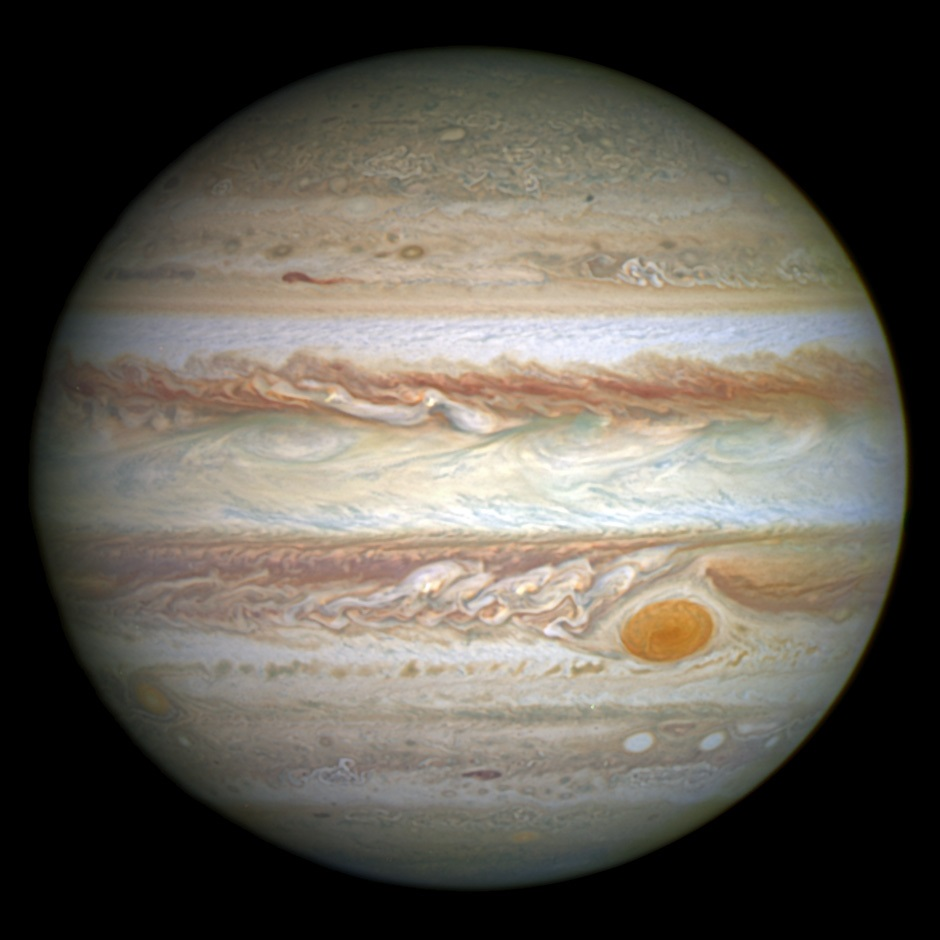
\includegraphics[width=0.9\linewidth]{images/book1/g6-jupiter-hubble.jpg}\\[2pt]
{\small Jupiter, difoto oleh Teleskop Antariksa Hubble pada tahun 2014.
(Foto: NASA, ESA, A.~Simon.)}
% ledger: hubble:jupiter-2014
\end{minipage}

\smallskip
{\small Kiri: massa jenis kedelapan planet; garis putus-putus adalah massa
jenis air. Kanan: yang kita lihat dari sebuah \omterm{def:g6:earth-a-planet:planet-types}{planet raksasa} adalah bagian
atas \omterm{def:g4:clouds-rain-snow:cloud}{awannya}.}
% ledger: planet:Mercury.density, planet:Venus.density, planet:Earth.density, planet:Mars.density, planet:Jupiter.density, planet:Saturn.density, planet:Uranus.density, planet:Neptune.density (figdata/grade-6/planets.py, part density)
\end{omfigure}

Foto Jupiter memperlihatkan pita-pita \omterm{def:g4:clouds-rain-snow:cloud}{awan}, terang dan gelap, serta sebuah
oval merah: Bintik Merah Raksasa, \omterm{def:g5:natural-hazards:storm}{badai} raksasa yang lebih besar daripada
seluruh Bumi, yang sudah bertiup selama ratusan tahun. Di bawah \omterm{def:g4:clouds-rain-snow:cloud}{awan} itu
tidak ada daratan: hanya gas, terutama hidrogen dan helium, yang makin ke
dalam makin padat.
% ledger: nasa:jupiter-gas

\begin{remark}[Planet yang lebih ringan daripada air]\label{rem:g6:earth-a-planet:saturn}
Saturnus adalah satu-satunya planet yang massa jenisnya lebih kecil daripada
massa jenis air: kira-kira 0.7~gram per sentimeter kubik. Seandainya ada
bak mandi yang cukup besar untuk menampungnya, Saturnus akan terapung!
% ledger: nasa:saturn-float, planet:Saturn.density
\end{remark}

\section{Seberapa jauh jarak antarplanet?}

Planet-planet tidak hanya sangat berbeda ukurannya; letaknya juga sangat
berjauhan satu sama lain. Bumi berjarak kira-kira 150~juta kilometer dari
Matahari. Neptunus, planet yang paling jauh, 30~kali lebih jauh: kira-kira
4500~juta kilometer. Gambar di bawah ini meletakkan kedelapan planet pada
satu garis, pada jaraknya masing-masing dari Matahari, menurut skala.
% ledger: planet:Earth.dist, planet:Neptune.dist

\begin{omfigure}
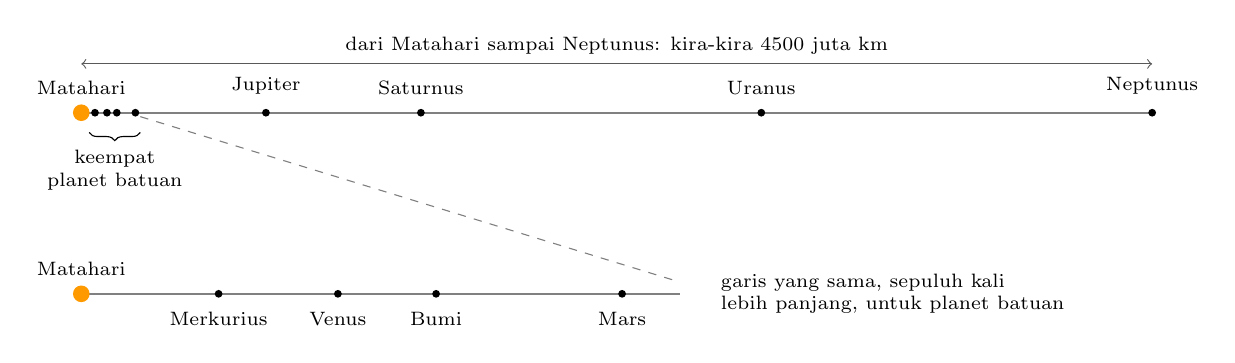
\begin{tikzpicture}
  % whole system
  \draw[thick, gray] (0,0) -- (13.6,0);
  \fill[orange!80!yellow] (0,0) circle (3pt);
  \node[font=\scriptsize, above=3pt] at (0,0) {Matahari};
  \foreach \n/\x/\lab in {Merkurius/0.174/, Venus/0.326/, Bumi/0.451/, Mars/0.687/,
                          Jupiter/2.345/Jupiter, Saturnus/4.313/Saturnus, Uranus/8.636/Uranus, Neptunus/13.6/Neptunus} {
    \fill (\x,0) circle (1.4pt);
    \node[font=\scriptsize, above=3pt] at (\x,0) {\lab};
  }
  \draw[decorate, decoration={brace, amplitude=3pt, mirror}] (0.1,-0.25) -- (0.75,-0.25)
    node[midway, below=3pt, font=\scriptsize, align=center] {keempat\\ planet batuan};
  \draw[<->, thin, gray!70!black] (0,0.62) -- (13.6,0.62) node[midway, above, font=\scriptsize, black] {dari Matahari sampai Neptunus: kira-kira 4500 juta km};
  % the inner system, ten times larger
  \begin{scope}[yshift=-2.3cm]
    \draw[thick, gray] (0,0) -- (7.6,0);
    \fill[orange!80!yellow] (0,0) circle (3pt);
    \node[font=\scriptsize, above=3pt] at (0,0) {Matahari};
    \foreach \n/\x in {Merkurius/1.744, Venus/3.259, Bumi/4.506, Mars/6.868} {
      \fill (\x,0) circle (1.4pt);
      \node[font=\scriptsize, below=3pt] at (\x,0) {\n};
    }
    \node[font=\scriptsize, anchor=west, align=left] at (8.0,0) {garis yang sama, sepuluh kali\\ lebih panjang, untuk planet batuan};
  \end{scope}
  \draw[dashed, gray] (0.75,-0.05) -- (7.6,-2.15);
\end{tikzpicture}

{\small Jarak planet-planet dari Matahari, menurut skala. Atas: seluruh Tata
Surya, dari Matahari sampai Neptunus. Bawah: keempat \omterm{def:g6:earth-a-planet:planet-types}{planet batuan},
diperbesar sepuluh kali. Ukuran titik-titiknya tidak menurut skala.}
% ledger: planet:Mercury.dist, planet:Venus.dist, planet:Earth.dist, planet:Mars.dist, planet:Jupiter.dist, planet:Saturn.dist, planet:Uranus.dist, planet:Neptune.dist (figdata/grade-6/planets.py, part dist)
\end{omfigure}

Keempat \omterm{def:g6:earth-a-planet:planet-types}{planet batuan} semuanya dekat dengan Matahari; keempat \omterm{def:g6:earth-a-planet:planet-types}{planet raksasa}
jauh di luar, dengan celah yang sangat lebar di antaranya. Celah antara
Mars dan Jupiter saja, kira-kira 550~juta kilometer, lebih dari dua kali
jarak dari Matahari ke Mars.
% ledger: planet:Mars.dist, planet:Jupiter.dist

Sulit menggambar ukuran dan jarak dengan skala yang sama: planet-planetnya
menjadi titik yang tidak terlihat. Sebuah \emph{model berskala} membantu
membayangkan keduanya sekaligus.

\begin{method}[Membuat model berskala Tata Surya]\label{met:g6:earth-a-planet:scale-model}
\begin{enumerate}
  \item Pilihlah ukuran Bumi dalam model, misalnya 1~cm.
  \item Carilah berapa kilometer sebenarnya yang diwakili oleh 1~cm pada
        model: bagilah diameter Bumi yang sebenarnya (12\,756~km) dengan
        ukurannya dalam model.
  \item Bagilah setiap ukuran sebenarnya dan setiap jarak sebenarnya dengan
        bilangan ini. Lalu ubahlah satuannya menjadi sesuatu yang mudah
        dibayangkan (sentimeter, meter, kilometer).
\end{enumerate}
% ledger: planet:Earth.diameter
\end{method}

\begin{example}[Kelereng sebagai Bumi]\label{ex:g6:earth-a-planet:marble}
Jika Bumi adalah sebuah kelereng selebar 1~cm, maka 1~cm mewakili
12\,756~km. Matahari, yang lebarnya 1\,391\,400~km, menjadi sebuah bola
selebar $1\,391\,400 \div 12\,756 \approx
109$~cm: bola yang lebih tinggi daripada anak kecil. Bumi berjarak
150~juta~km dari Matahari: $149\,600\,000 \div 12\,756 \approx 11\,700$~cm,
yaitu kira-kira 117~meter, sepanjang lapangan sepak bola.
% ledger: planet:Earth.diameter, sun:R, planet:Earth.dist
\end{example}

\begin{center}\small
\begin{tabular}{|l|c|c|}
\hline
\textbf{benda langit} & \textbf{ukuran dalam model (cm)} & \textbf{jarak dari Matahari (m)} \\
\hline
Matahari & 109 & --- \\
Merkurius & 0.38 & 45 \\
Venus & 0.95 & 85 \\
Bumi & 1.00 & 117 \\
Mars & 0.53 & 179 \\
Jupiter & 11.21 & 610 \\
Saturnus & 9.45 & 1123 \\
Uranus & 4.01 & 2248 \\
Neptunus & 3.88 & 3540 \\
\hline
\end{tabular}
\end{center}
% ledger: sun:R, planet:Mercury.diameter, planet:Venus.diameter, planet:Earth.diameter, planet:Mars.diameter, planet:Jupiter.diameter, planet:Saturn.diameter, planet:Uranus.diameter, planet:Neptune.diameter, planet:Mercury.dist, planet:Venus.dist, planet:Earth.dist, planet:Mars.dist, planet:Jupiter.dist, planet:Saturn.dist, planet:Uranus.dist, planet:Neptune.dist (figdata/grade-6/planets.py, part model)

Dalam model ini, seluruh Tata Surya sampai Neptunus terbentang di atas
sebuah lingkaran selebar 7~km, dengan sebuah bola besar di tengahnya dan
delapan kelereng dan bola, yang terbesar seukuran jeruk bali, yang
tersebar di dalamnya. Tata Surya sebagian besar berupa ruang kosong.

\section{Venus, Bumi, dan Mars}

Venus, Bumi, dan Mars bertetangga, dan ketiganya \omterm{def:g6:earth-a-planet:planet-types}{planet batuan}. Venus
hampir sama besarnya dengan Bumi: diameternya 95~\% diameter Bumi. Mars
lebih kecil: diameternya kira-kira separuh diameter Bumi. Akan tetapi,
ketiga planet ini sangat berbeda satu sama lain.
% ledger: planet:Venus.diameter, planet:Earth.diameter, planet:Mars.diameter (planets.py: 94.9 %)

\paragraph{Venus.} Venus terbungkus lapisan udara yang tebal, yang sebagian
besar terdiri atas karbon dioksida, dengan \omterm{def:g4:clouds-rain-snow:cloud}{awan} asam sulfat yang tebal,
sejenis asam yang membakar. Udaranya begitu tebal sehingga menekan tanah
92~kali lebih kuat daripada udara Bumi menekan tanah kita. Di permukaannya,
suhunya kira-kira 464~$^\circ$C: cukup panas untuk melelehkan timah hitam.
Tidak ada air yang dapat tetap cair di sana.
% ledger: nasa:venus-clouds, planet:Venus.psurf, planet:Venus.Tmean

\paragraph{Mars.} Mars adalah \omterm{def:g5:weather-and-climate:desert}{gurun} yang dingin, kering, dan berdebu.
Udaranya juga sebagian besar terdiri atas karbon dioksida, tetapi sangat
tipis: udara itu menekan tanah kira-kira seratus kali lebih lemah daripada
udara Bumi. Suhu rata-ratanya $-65$~$^\circ$C. Saat ini memang ada air di
sana, tetapi dalam keadaan membeku: sebagai es di tudung \omterm{def:g3:continents-and-oceans:poles}{kutub} dan di bawah
tanah dekat \omterm{def:g3:continents-and-oceans:poles}{kutub}. Akan tetapi, Mars tidak selalu seperti ini: miliaran
tahun yang lalu, \omterm{def:g1:landscapes-around-us:water}{sungai-sungai} mengalir di Mars, \omterm{def:g1:landscapes-around-us:water}{danau-danau} terbentuk, dan
\omterm{def:g5:water-shapes-the-land:flood}{banjir} melanda permukaannya.
% ledger: nasa:mars-water, planet:Mars.psurf, planet:Mars.Tmean

\paragraph{Bumi.} Di antara keduanya, Bumi mempunyai udara yang menekan
tanah dengan kira-kira 1~bar (satuan yang dipakai untuk membandingkan
tekanan udara di planet-planet), suhu rata-rata 15~$^\circ$C, dan \omterm{def:g2:water-on-earth:ocean}{samudra}
berisi air cair.
% ledger: planet:Earth.psurf, planet:Earth.Tmean

\begin{omfigure}
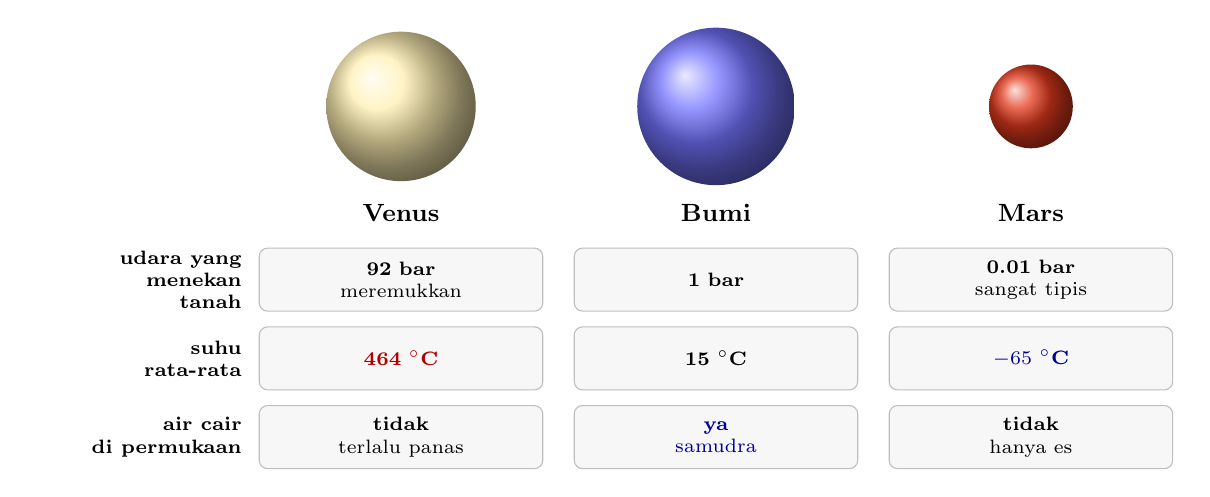
\begin{tikzpicture}[x=1cm, y=1cm,
    lab/.style={font=\scriptsize, align=center, text width=3.6cm},
    row/.style={font=\scriptsize\bfseries, anchor=east, align=right, text width=2.6cm}]
  % discs to scale: diameters 94.9 %, 100 %, 53.2 % of the Earth's (planets.py)
  \shade[ball color=yellow!60!orange!30] (3,0) circle (0.949);
  \shade[ball color=blue!55] (7,0) circle (1.0);
  \shade[ball color=red!55!brown] (11,0) circle (0.532);
  \node[font=\small\bfseries] at (3,-1.35) {Venus};
  \node[font=\small\bfseries] at (7,-1.35) {Bumi};
  \node[font=\small\bfseries] at (11,-1.35) {Mars};
  \foreach \y/\t in {-2.2/{udara yang menekan\\tanah}, -3.2/{suhu\\rata-rata},
                     -4.2/{air cair\\di permukaan}}
    {\node[row] at (1.1,\y) {\t};}
  \foreach \x in {3,7,11}{
    \foreach \y in {-2.2,-3.2,-4.2}{
      \draw[rounded corners=3pt, black!25, fill=black!3] (\x-1.8,\y-0.4) rectangle (\x+1.8,\y+0.4);}}
  \node[lab] at (3,-2.2) {\textbf{92 bar}\\meremukkan};
  \node[lab] at (7,-2.2) {\textbf{1 bar}};
  \node[lab] at (11,-2.2) {\textbf{0.01 bar}\\sangat tipis};
  \node[lab, text=red!70!black] at (3,-3.2) {\textbf{464~$^\circ$C}};
  \node[lab] at (7,-3.2) {\textbf{15~$^\circ$C}};
  \node[lab, text=blue!60!black] at (11,-3.2) {\textbf{$-65$~$^\circ$C}};
  \node[lab] at (3,-4.2) {\textbf{tidak}\\terlalu panas};
  \node[lab, text=blue!60!black] at (7,-4.2) {\textbf{ya}\\samudra};
  \node[lab] at (11,-4.2) {\textbf{tidak}\\hanya es};
\end{tikzpicture}

{\small Venus, Bumi, dan Mars dibandingkan. Ketiga cakram itu digambar
menurut skala. (Nilai: lembar fakta planet NASA.)}
% ledger: planet:Venus.psurf, planet:Earth.psurf, planet:Mars.psurf, planet:Mercury.Tmean, planet:Venus.Tmean, planet:Earth.Tmean, planet:Mars.Tmean, planet:Jupiter.Tmean, planet:Saturn.Tmean, planet:Uranus.Tmean, planet:Neptune.Tmean, nasa:mars-water
\end{omfigure}

\paragraph{Panas dan dingin.} Di dekat Matahari, sebuah planet menerima
banyak cahaya dan panasnya; jauh dari Matahari, sangat sedikit. Jadi makin
jauh sebuah planet dari Matahari, seharusnya makin dingin planet itu. Diagram
di bawah ini menunjukkan bahwa hal ini benar mulai dari Bumi ke luar:
planet-planet raksasa, yang letaknya jauh, adalah dunia yang membeku. Akan
tetapi, lihatlah Venus: jaraknya dari Matahari hampir dua kali jarak
Merkurius, tetapi Venus lebih panas! Udaranya yang tebal, yang terdiri atas
karbon dioksida, menahan panas Matahari seperti selimut tebal dan tidak
membiarkannya lepas. Merkurius, yang hampir tidak berudara, tidak dapat
menyimpan panasnya.
% ledger: planet:Mercury.Tmean, planet:Venus.Tmean, planet:Earth.Tmean, planet:Mars.Tmean, planet:Jupiter.Tmean, planet:Saturn.Tmean, planet:Uranus.Tmean, planet:Neptune.Tmean, planet:Mercury.dist, planet:Venus.dist, planet:Earth.dist, planet:Mars.dist, planet:Jupiter.dist, planet:Saturn.dist, planet:Uranus.dist, planet:Neptune.dist, nasa:venus-clouds, planet:Mercury.psurf

\begin{omfigure}
\begin{tikzpicture}
  \begin{axis}[ybar, bar width=14pt, width=0.86\linewidth, height=6cm,
      ymin=-270, ymax=520, xmin=-0.6, xmax=7.6,
      xtick={0,...,7},
      xticklabels={{Merkurius\\58}, {Venus\\108}, {Bumi\\150}, {Mars\\228},
                   {Jupiter\\779}, {Saturnus\\1432}, {Uranus\\2867}, {Neptunus\\4515}},
      xticklabel style={align=center, font=\scriptsize},
      axis x line*=bottom, axis y line*=left,
      xticklabel pos=lower, ytick={-200,-100,...,500},
      ylabel={suhu rata-rata ($^\circ$C)}, xlabel={planet dan jarak dari Matahari (juta km)},
      tick label style={font=\scriptsize}, label style={font=\scriptsize},
      nodes near coords, nodes near coords style={font=\tiny},
      every node near coord/.append style={/pgf/number format/1000 sep={}}]
    \addplot[fill=orange!50, draw=black!60, bar shift=0pt]
      table[x=idx, y=tmean_C] {figdata/out/grade-6-planets-temp.dat};
    \draw[black!50] (axis cs:-0.6,0) -- (axis cs:7.6,0);
  \end{axis}
\end{tikzpicture}

{\small Suhu rata-rata planet-planet, menurut urutan jaraknya dari Matahari.
Venus melanggar aturan itu: Venus lebih panas daripada Merkurius, yang
lebih dekat dengan Matahari. (Nilai: lembar fakta planet NASA.)}
% ledger: planet:Mercury.Tmean, planet:Venus.Tmean, planet:Earth.Tmean, planet:Mars.Tmean, planet:Jupiter.Tmean, planet:Saturn.Tmean, planet:Uranus.Tmean, planet:Neptune.Tmean, planet:Mercury.dist, planet:Venus.dist, planet:Earth.dist, planet:Mars.dist, planet:Jupiter.dist, planet:Saturn.dist, planet:Uranus.dist, planet:Neptune.dist (figdata/grade-6/planets.py, part temp)
\end{omfigure}

\section{Apa yang membuat kehidupan mungkin ada di Bumi}

Bumi adalah satu-satunya planet yang kita ketahui memiliki kehidupan.
Makhluk hidup memerlukan beberapa syarat sekaligus, dan Bumi memiliki
semuanya.

\begin{itemize}
  \item \textbf{Air cair.} Semua makhluk hidup memerlukan air cair: Bumi
        mempunyai \omterm{def:g2:water-on-earth:ocean}{samudra}, \omterm{def:g1:landscapes-around-us:water}{sungai}, dan \omterm{def:g1:landscapes-around-us:water}{danau}.
  \item \textbf{Suhu yang sedang.} Di permukaan Bumi, air membeku pada
        0~$^\circ$C dan mendidih pada 100~$^\circ$C (fisika). Dengan
        rata-rata 15~$^\circ$C, suhu Bumi sebagian besar tetap berada di
        antara keduanya, sehingga airnya tetap cair.
  \item \textbf{Jarak yang tepat dari Matahari.} Jika lebih dekat dengan
        Matahari, seperti Venus, sebuah planet bisa menjadi terlalu panas;
        jika lebih jauh, seperti Mars, terlalu dingin. Bumi berada pada jarak
        yang tepat untuk air cair.
  \item \textbf{Atmosfer.} Lapisan udara di sekeliling Bumi menjaga
        permukaannya tetap hangat pada malam hari, memberi makhluk hidup
        gas yang mereka perlukan, dan cukup menekan \omterm{def:g2:water-on-earth:ocean}{samudra} agar airnya
        tetap cair. Di Mars, udaranya begitu tipis sehingga air cair tidak
        dapat bertahan lama di permukaan: air itu membeku atau berubah
        menjadi uap.
\end{itemize}
% ledger: nasa:mars-water, planet:Earth.Tmean

\begin{remark}[Pernahkah ada kehidupan di Mars?]\label{rem:g6:earth-a-planet:mars-life}
Karena Mars dulu mempunyai \omterm{def:g1:landscapes-around-us:water}{sungai} dan \omterm{def:g1:landscapes-around-us:water}{danau}, para ilmuwan bertanya-tanya
apakah makhluk hidup yang sangat kecil pernah hidup di sana, dahulu kala,
ketika Mars lebih hangat dan basah. Para ilmuwan tidak berharap menemukan
makhluk hidup di Mars saat ini; dengan robot penjelajah, mereka mencari di
dalam \omterm{def:g3:stones-pebbles-sand:rock}{batuannya} tanda-tanda kehidupan yang pernah ada dahulu kala.
% ledger: nasa:mars-water
\end{remark}

\section{Bumi dilihat dari antariksa}

Selama ribuan tahun, manusia hanya dapat membayangkan seperti apa planetnya
jika dilihat dari luar. Pada tanggal 24~Desember~1968, para astronaut
Apollo~8, yang mengorbit Bulan, melihat Bumi terbit di atas cakrawala Bulan
yang kelabu, dan salah seorang dari mereka, Bill Anders, mengambil foto di
bawah ini.
% ledger: nasa:earthrise

\begin{omfigure}
\begin{minipage}[c]{0.46\linewidth}\centering
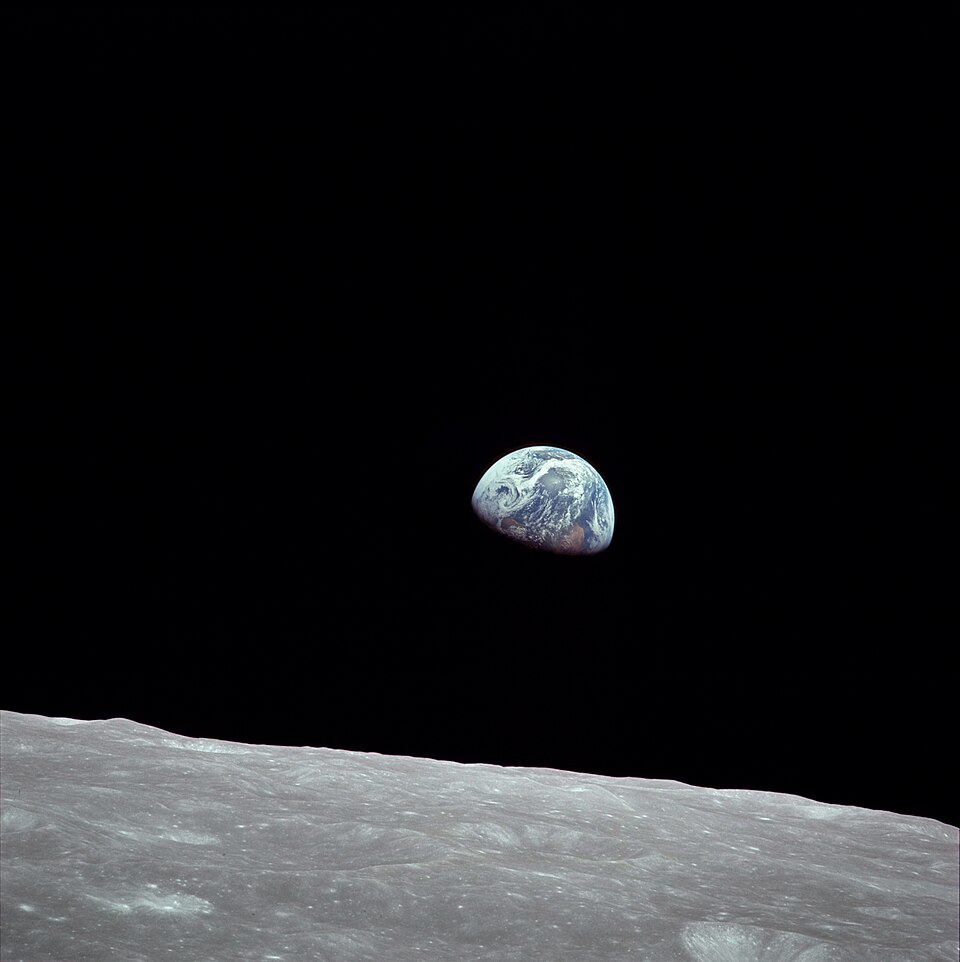
\includegraphics[width=0.85\linewidth]{images/book1/g6-earthrise.jpg}
\end{minipage}\hfill
\begin{minipage}[c]{0.5\linewidth}
{\small \emph{Earthrise} (Bumi terbit): Bumi di atas cakrawala Bulan, difoto
dari Apollo~8 yang mengorbit Bulan, 24~Desember~1968.
(Foto: NASA, Bill Anders.)}

\medskip
{\small Perhatikan warna-warnanya: biru \omterm{def:g2:water-on-earth:ocean}{samudra}, pusaran putih \omterm{def:g4:clouds-rain-snow:cloud}{awan}, cokelat
daratan. Di sekelilingnya, hitamnya antariksa; di latar depan, tanah Bulan
yang kelabu dan mati, tanpa air dan tanpa udara.}
\end{minipage}
% ledger: nasa:earthrise
\end{omfigure}

Dilihat dari antariksa, Bumi sebagian besar berwarna biru: \omterm{def:g2:water-on-earth:ocean}{samudra} menutupi
kira-kira tujuh persepuluh permukaannya. \omterm{def:g4:clouds-rain-snow:cloud}{Awan} putih yang tersusun dari titik
air berpusar di atasnya, dan es putih menutupi \omterm{def:g3:continents-and-oceans:poles}{kutub-kutubnya}. Daratan
berwarna cokelat di tempat yang kering, hijau di tempat tumbuhan tumbuh.
Udara itu sendiri tidak dapat dilihat, tetapi \omterm{def:g4:clouds-rain-snow:cloud}{awan} yang melayang di
dalamnya menunjukkan bahwa udara itu ada. Di antara semua planet di Tata
Surya, hanya Bumi yang menampilkan warna-warna ini bersama-sama: air cair,
\omterm{def:g4:clouds-rain-snow:cloud}{awan}, dan tumbuhan yang hidup.
% ledger: wss:ocean-cover, nasa:apollo17-earth

\begin{history}[Titik biru pucat]
\begin{minipage}[c]{0.66\linewidth}
Pada tanggal 14~Februari~1990, wahana antariksa Voyager~1 berada kira-kira
6~miliar kilometer dari Matahari, lebih jauh daripada Neptunus. Sebelum
meninggalkan Tata Surya, wahana itu memutar kameranya ke belakang dan
memotret Bumi. Di dalam foto itu, planet kita hanyalah sebuah bintik
terang, lebih kecil daripada sebutir debu, yang tertangkap dalam seberkas
sinar matahari. Ahli astronomi Carl Sagan menulis tentang foto itu:
``Lihatlah lagi titik itu. Itulah tempat ini. Itulah rumah kita. Itulah
kita.''
% ledger: nasa:pale-blue-dot
\end{minipage}\hfill
\begin{minipage}[c]{0.3\linewidth}\centering
\begin{tikzpicture}
  \node[inner sep=0] (img) {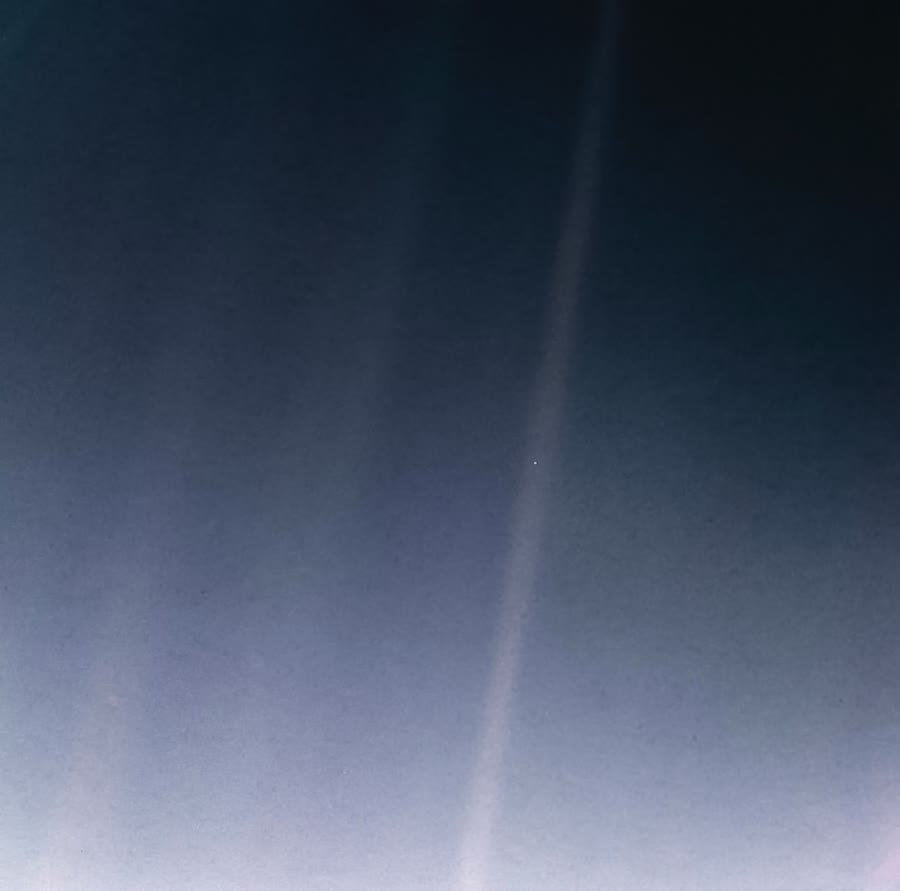
\includegraphics[width=\linewidth]{images/book1/g6-pale-blue-dot.jpg}};
  \draw[yellow!80!orange, thick] ($(img.south west)!0.594!(img.south east) + (0,{0.476*\linewidth})$) circle (6pt);
\end{tikzpicture}\\[2pt]
{\footnotesize Bumi (dilingkari) dilihat oleh Voyager~1, 1990. (Gambar:
NASA/JPL-Caltech, domain publik.)}
% ledger: nasa:pale-blue-dot
\end{minipage}
\end{history}

\section{Latihan}

\begin{exercise}[$\star$]\label{exo:g6:earth-a-planet:1}
Tuliskan kedelapan planet Tata Surya secara berurutan, dari yang paling
dekat dengan Matahari sampai yang paling jauh. Garis bawahi planet-planet
\omterm{def:g3:stones-pebbles-sand:rock}{batuan}.
\end{exercise}

\begin{exercise}[$\star$]\label{exo:g6:earth-a-planet:2}
Salin dan lengkapi: ``\omterm{def:g6:earth-a-planet:planet-types}{Planet batuan} itu kecil dan \ldots, dengan permukaan
yang \ldots{} \omterm{def:g6:earth-a-planet:planet-types}{Planet raksasa} itu sangat besar, dengan \ldots{} yang rendah,
sebagian besar tersusun dari \ldots{} dan \ldots{}''
\end{exercise}

\begin{exercise}[$\star$]\label{exo:g6:earth-a-planet:3}
Dengan memakai tabel dalam bab ini, planet manakah yang diameternya paling
mendekati diameter Bumi? Planet manakah yang paling besar? Planet manakah
yang paling kecil?
\end{exercise}

\begin{exercise}[$\star$]\label{exo:g6:earth-a-planet:4}
Benar atau salah? Perbaiki kalimat yang salah.
(a) Venus tertutup \omterm{def:g2:water-on-earth:ocean}{samudra}.
(b) Mars lebih dingin daripada Bumi.
(c) Planet-planet raksasa adalah keempat planet yang paling dekat dengan Matahari.
(d) Massa jenis Saturnus lebih kecil daripada massa jenis air.
\end{exercise}

\begin{exercise}[$\star\star$]\label{exo:g6:earth-a-planet:5}
Diameter Merkurius adalah 4\,879~km, diameter Bumi 12\,756~km. Hitunglah
diameter Merkurius sebagai persentase dari diameter Bumi, dibulatkan ke
bilangan bulat terdekat.
% ledger: planet:Mercury.diameter, planet:Earth.diameter (planets.py: 38.2 %)
\end{exercise}

\begin{exercise}[$\star\star$]\label{exo:g6:earth-a-planet:6}
Berapa Bumi, yang dijajarkan berdampingan, yang muat di sepanjang diameter
Saturnus (120\,536~km)? Bulatkan ke bilangan bulat terdekat. Apakah
Saturnus \omterm{def:g6:earth-a-planet:planet-types}{planet batuan} atau \omterm{def:g6:earth-a-planet:planet-types}{planet raksasa}?
% ledger: planet:Saturn.diameter, planet:Earth.diameter
\end{exercise}

\begin{exercise}[$\star\star$]\label{exo:g6:earth-a-planet:7}
Para ahli astronomi telah menemukan planet-planet yang mengelilingi bintang
lain. Planet~A mempunyai massa jenis 1.1~gram per sentimeter kubik dan
9~kali lebih lebar daripada Bumi. Planet~B mempunyai massa jenis 5.0~gram
per sentimeter kubik dan sedikit lebih kecil daripada Bumi. Manakah yang
merupakan \omterm{def:g6:earth-a-planet:planet-types}{planet batuan} dan manakah yang merupakan \omterm{def:g6:earth-a-planet:planet-types}{planet raksasa}?
Jelaskan.
\end{exercise}

\begin{exercise}[$\star\star$]\label{exo:g6:earth-a-planet:8}
Dengan memakai diagram suhu planet-planet: (a) berapa derajat Venus lebih
panas daripada Bumi? (b) Berapa derajat Mars lebih dingin daripada Bumi?
% ledger: planet:Venus.Tmean, planet:Earth.Tmean, planet:Mars.Tmean
\end{exercise}

\begin{exercise}[$\star\star$]\label{exo:g6:earth-a-planet:9}
Merkurius adalah planet yang paling dekat dengan Matahari, tetapi Venus yang
paling panas. Jelaskan sebabnya.
\end{exercise}

\begin{exercise}[$\star\star$]\label{exo:g6:earth-a-planet:10}
Bumi berjarak 150~juta kilometer dari Matahari dan Mars 228~juta kilometer.
Berapa juta kilometer Mars lebih jauh dari Matahari? Berapa persen jarak
Mars lebih besar daripada jarak Bumi (bulatkan ke bilangan bulat terdekat)?
% ledger: planet:Earth.dist, planet:Mars.dist
\end{exercise}

\begin{exercise}[$\star\star\star$]\label{exo:g6:earth-a-planet:11}
Seorang teman berkata: ``Mars selalu menjadi \omterm{def:g5:weather-and-climate:desert}{gurun} yang kering; di sana
tidak pernah ada air.'' Dengan memakai bab ini, jawablah dia: apa yang
dimiliki Mars miliaran tahun yang lalu, di mana airnya sekarang, dan mengapa
air cair tidak dapat bertahan di permukaannya sekarang?
\end{exercise}

\begin{exercise}[$\star\star\star$]\label{exo:g6:earth-a-planet:12}
Venus kadang-kadang disebut kembaran Bumi. Diameternya 95~\% diameter
Bumi, dan tarikan gravitasi di permukaannya 8.9 pada skala yang nilainya
9.8 untuk Bumi. (a) Hitunglah tarikan gravitasi Venus sebagai persentase
dari tarikan gravitasi Bumi,
dibulatkan ke bilangan bulat terdekat. (b) Sebutkan dua hal yang membuat
Venus seperti kembaran Bumi, dan dua hal yang membuatnya tidak seperti itu.
% ledger: planet:Venus.gravity, planet:Earth.gravity, planet:Venus.diameter
\end{exercise}

\section{Soal: Kartu Pos dari Tiga Planet}

\begin{problem}[{Soal akhir pekan --- tiga kartu pos dari antariksa, dan
seberapa kuat udara Venus menekan tanahnya}]
\label{pb:g6:earth-a-planet:1}
% ledger: planet:Venus.dist, planet:Venus.diameter, planet:Venus.density, planet:Venus.Tmean, planet:Venus.psurf, planet:Earth.dist, planet:Earth.diameter, planet:Earth.density, planet:Earth.Tmean, planet:Earth.psurf, planet:Mars.dist, planet:Mars.diameter, planet:Mars.density, planet:Mars.Tmean, planet:Mars.psurf, nasa:venus-clouds, nasa:mars-water
Tiga wahana robot masing-masing mengirimkan sebuah kartu pos ke Bumi, dengan
beberapa angka yang tertulis di baliknya.

\begin{center}
\small
\begin{tabular}{>{\raggedright\arraybackslash}p{0.29\linewidth}>{\raggedright\arraybackslash}p{0.29\linewidth}>{\raggedright\arraybackslash}p{0.29\linewidth}}
\hline
\textbf{Dari Venus} & \textbf{Dari Bumi} & \textbf{Dari Mars}\\
\hline
Jarak dari Matahari: 108~juta~km. & Jarak dari Matahari:
150~juta~km. & Jarak dari Matahari: 228~juta~km.\\
Diameter: 12\,104~km. & Diameter: 12\,756~km. & Diameter: 6\,792~km.\\
Massa jenis: 5.2~g/cm$^3$. & Massa jenis: 5.5~g/cm$^3$. & Massa jenis: 3.9~g/cm$^3$.\\
Suhu rata-rata: 464~$^\circ$C. & Suhu rata-rata: 15~$^\circ$C. &
Suhu rata-rata: $-65$~$^\circ$C.\\
Udara menekan tanah dengan 92~bar. \omterm{def:g4:clouds-rain-snow:cloud}{Awan} asam yang tebal. &
Udara menekan tanah dengan 1~bar. \omterm{def:g2:water-on-earth:ocean}{Samudra} dan \omterm{def:g4:clouds-rain-snow:cloud}{awan}. &
Udara menekan tanah dengan 0.01~bar. Es di \omterm{def:g3:continents-and-oceans:poles}{kutub}.\\
\hline
\end{tabular}
\end{center}

\medskip
\noindent\textbf{Bagian I --- Membandingkan planet-planet.}
\begin{enumerate}
  \item Urutkan ketiga planet itu menurut jaraknya dari Matahari.
  \item Berapa juta kilometer Venus lebih dekat dengan Matahari daripada
        Bumi? Berapa juta kilometer Mars lebih jauh?
  \item Hitunglah diameter Mars sebagai persentase dari diameter Bumi,
        dibulatkan ke bilangan bulat terdekat. Apakah lebar Mars kira-kira
        seperempat, separuh, atau tiga perempat lebar Bumi?
  \item Apakah ketiga planet itu \omterm{def:g6:earth-a-planet:planet-types}{planet batuan} atau \omterm{def:g6:earth-a-planet:planet-types}{planet raksasa}? Angka
        mana pada kartu pos yang memberitahumu hal itu?
\end{enumerate}

\medskip
\noindent\textbf{Bagian II --- Udara.}
\begin{enumerate}[resume]
  \item Di planet manakah udaranya paling tebal? Di planet manakah udaranya
        paling tipis?
  \item Berapa kali lebih lemah udara Mars menekan tanahnya dibandingkan
        dengan udara Bumi menekan tanah kita?
  \item Venus lebih dekat dengan Matahari daripada Bumi, tetapi hal itu saja
        tidak menjelaskan suhu 464~$^\circ$C. Apa yang dilakukan udara Venus
        terhadap panas Matahari?
  \item Berapa kali lebih kuat udara menekan tanah Venus dibandingkan dengan
        di Bumi? Mengapa wahana yang mendarat di Venus harus mempunyai dinding yang sangat kuat?
\end{enumerate}

\medskip
\noindent\textbf{Bagian III --- Air dan kehidupan.}
\begin{enumerate}[resume]
  \item Di permukaan Bumi, air membeku pada 0~$^\circ$C dan mendidih pada
        100~$^\circ$C. Dengan memakai suhu rata-rata, jelaskan mengapa air
        berwujud cair di Bumi.
  \item Apa yang akan terjadi pada segelas air yang diletakkan di tanah
        Venus? Di tanah Mars?
  \item Mars mempunyai \omterm{def:g1:landscapes-around-us:water}{sungai} dan \omterm{def:g1:landscapes-around-us:water}{danau} miliaran tahun yang lalu. Apa yang
        diberitahukan hal ini kepada kita tentang \omterm{def:g5:weather-and-climate:climate}{iklim} Mars dahulu kala,
        dibandingkan dengan sekarang?
  \item Tuliskan bagian belakang kartu pos dari Bumi: dalam beberapa kalimat,
        sebutkan empat alasan mengapa kehidupan mungkin ada di Bumi.
\end{enumerate}
\end{problem}
